\chapter{Laboratorio de pruebas}

% **************************** Define Graphics Path **************************
\ifpdf
    \graphicspath{{Chapter6/Figs/Raster/}{Chapter6/Figs/PDF/}{Chapter6/Figs/}}
\else
    \graphicspath{{Chapter6/Figs/Vector/}{Chapter6/Figs/}}
\fi

Para validar funcionalmente el prototipo es preciso la construcción de un laboratorio de experimentación sobre el cual ejecutar un conjunto de pruebas e implementar algunos casos de uso representativos. Dentro de las pruebas funcionales se busca verificar aspectos importantes de la implementaci\'on como la clasificación de tr\'afico, el algoritmo de ruteo dinámico y el algoritmo de distribución de etiquetas.

Por otro lado con la implementaci\'on de algunos casos de uso representativos se busca validar la utilización del enfoque OpenFlow/SDN en la construcci\'on a futuro de la RAU2.\\

El siguiente capitulo esta destinado a la presentación del laboratorio de pruebas construido y a la descripción de las diferentes pruebas realizadas.

% **************************** Construccion del TestBed ************************** 
\section{Definición del Laboratorio}

Como se menciona anteriormente uno de los objetivos de este laboratorio de experimentaci\'on es verificar el correcto funcionamiento de la implementaci\'on realizada, en particular en los aspectos críticos de la misma como la capacidad para clasificar trafico y los diferentes algoritmos de ruteo, distribución de etiquetas, actualización topologica, etc. 

Para esto es necesario construir un prototipo con suficientes nodos y enlaces como para poder definir varios servicios de redes privadas. Tambi\'en interesa la existencia de caminos alternativos entre un par de nodos origen y destino para poder comprobar el funcionamiento del algoritmo de ruteo y evaluar el comportamiento del prototipo cuando la topolog\'ia cambia, desconectando enlaces, apagando nodos, etc.\\

Teniendo en cuanta los requerimientos mencionados se construye un laboratorio de pruebas con la siguiente topolog\'ia (ver figura \ref{fig:LaboratorioDePruebasTopo}).
  
\begin{figure}[ht!] 
\centering    
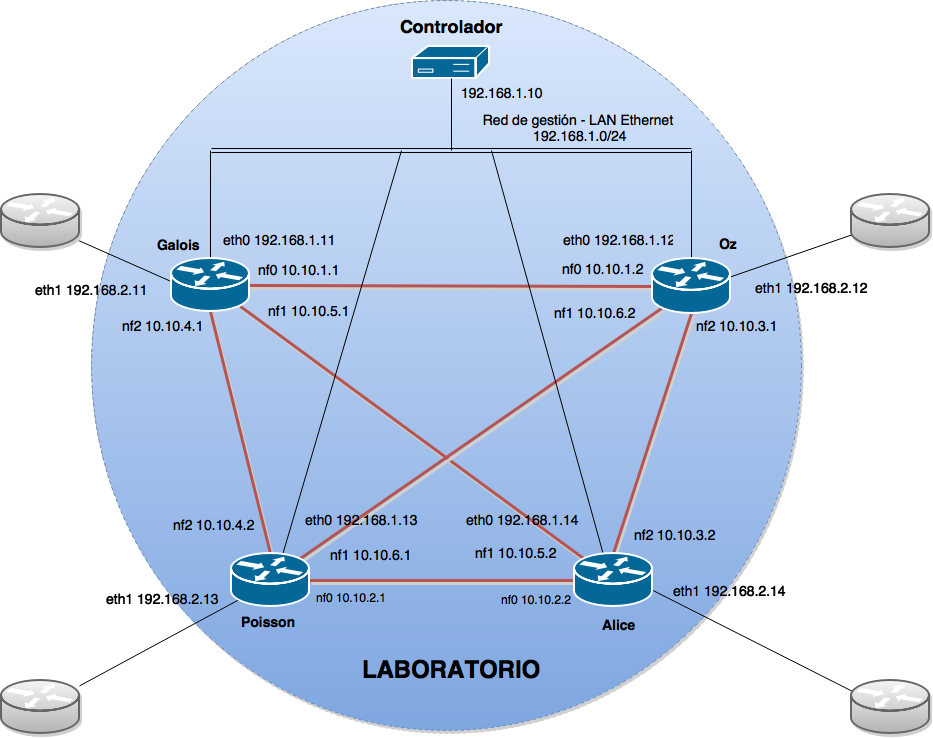
\includegraphics[width=0.85\textwidth]{Topologia}
\caption[Laboratorio de pruebas - Topolog\'ia]{Laboratorio de pruebas - Topolog\'ia}
\label{fig:LaboratorioDePruebasTopo}
\end{figure}

El laboratorio se compone de cuatro nodos implementados en base al dispositivo RAU-Switch conectados entre si con enlaces de fibra \'optica multimodo. Cada nodo esta conectado a los otros tres nodos de la topolog\'ia implementando de esta forma una topolog\'ia full mesh de cuatro nodos.

A su vez cada nodo esta conectado al controlador SDN del prototipo mediante una interfaz de red de 10Mb (interfaces \textbf{eth0}).\\

Por la forma que tiene la topolog\'ia, los cuatro nodos nombrados \textit{Galois}, \textit{Poisson}, \textit{Oz} y \textit{Alice} son nodos de borde. Esto quiere decir que RAUFlow los considera como nodos habilitados para ser nodo de ingreso \'o nodo de egreso en la definici\'on de servicios de redes privadas.

Por otro lado cada nodo cuenta con una interfaz de red de 100Mb (interfaz \textbf{eth1}) utilizada como interfaz externa para la conexi\'on con otras subredes. Estas interfaces son utilizadas por RAUFlow para la definici\'on de servicios de VPN como los puntos de entrada y salida de tr\'afico. Por tanto cada una de estas interfaces se encuentra directamente conectada a la subred de una VPN en particular.\\  

Como se menciona anteriormente en lacp\'itulo 5, la representaci\'on utilizada para modelar una topolog\'ia de red es la de un multigrafo dirigido ponderado. En la figura \ref{fig:LaboratorioDePruebasCostos} se muestra esta representaci\'on para la topolog\'ia del prototipo. Como puede apreciarse en la im\'agen cada enlace tiene su respectivo costo asociado.

Por simplicidad en el diagrama se han obviado los enlaces existentes entre el Controlador y cada uno de los nodos. Como se menciona en el cap\'itulo 4 la instancia de Quagga ejecutada en el controlador tiene como \'unico objetivo contar con un acceso local a la LSDB. Por ello conceptualmente el costo asociado a cada uno de estos enlaces es infinito, lo cual en pr\'actica se realiza asignando el valor 65535.  

\begin{figure}[ht!] 
\centering    
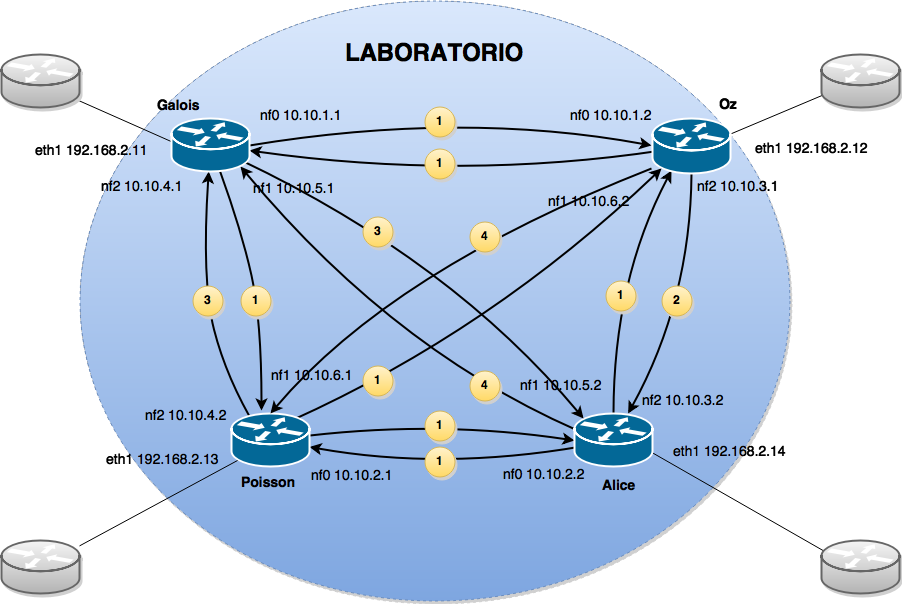
\includegraphics[width=0.85\textwidth]{TopologiaCostos}
\caption[Laboratorio de pruebas - Costos de la topolog\'ia]{Laboratorio de pruebas - Costos de la topolog\'ia}
\label{fig:LaboratorioDePruebasCostos}
\end{figure}

Sobre este laboratorio se implementan dos casos de uso representativos: (a) VPN de capa 3 y (b) VPN de capa 2. Sobre cada uno de estos casos de uso a su vez se ejecutan una serie de pruebas orientadas a verificar el correcto funcionamiento de las componentes m\'as importantes en la implementaci\'on de RAUFlow y RAU-Switch.

A continuaci\'on se describen los resultados obtenidos en la implementaci\'on de estos casos de uso y la eecuci\'on de estas pruebas, comenzando por el caso de uso VPN de capa 3.

\section{VPN de capa 3}

Las redes privadas virtuales de capa 3 son un tipo de servicio comunmente brindado por un operador de red y es en particular uno de los servicios que se quiere implementar en la RAU2. En particular con este tipo de red privada se puede implementar clasificaci\'on de tr\'afico en base a tipo de aplicaci\'on y numeraci\'on de capa 3.\\

En este trabajo se implementan dos escenarios diferentes para este tipo de red privada: (a) red privada multipunto con una \'unica organizaci\'on y tres sucursales f\'isicamente separadas, (b) red privada punto a punto con dos organizaciones, cada una de ellas con dos sucursales f\'isicamente separadas.

\subsection{Escenario 1 - Red Privada Multipunto}

Este escenario representa una red privada multipunto de capa 3. Esta compuesto por una \'unica organizaci\'on o red privada dividida en 3 sucursales o subredes.

Se quiere instanciar entonces servicios en RAUFlow con el obetivo de brindar conectividad entre las 3 sucursales de la organizaci\'on.

\begin{figure}[ht!] 
\centering    
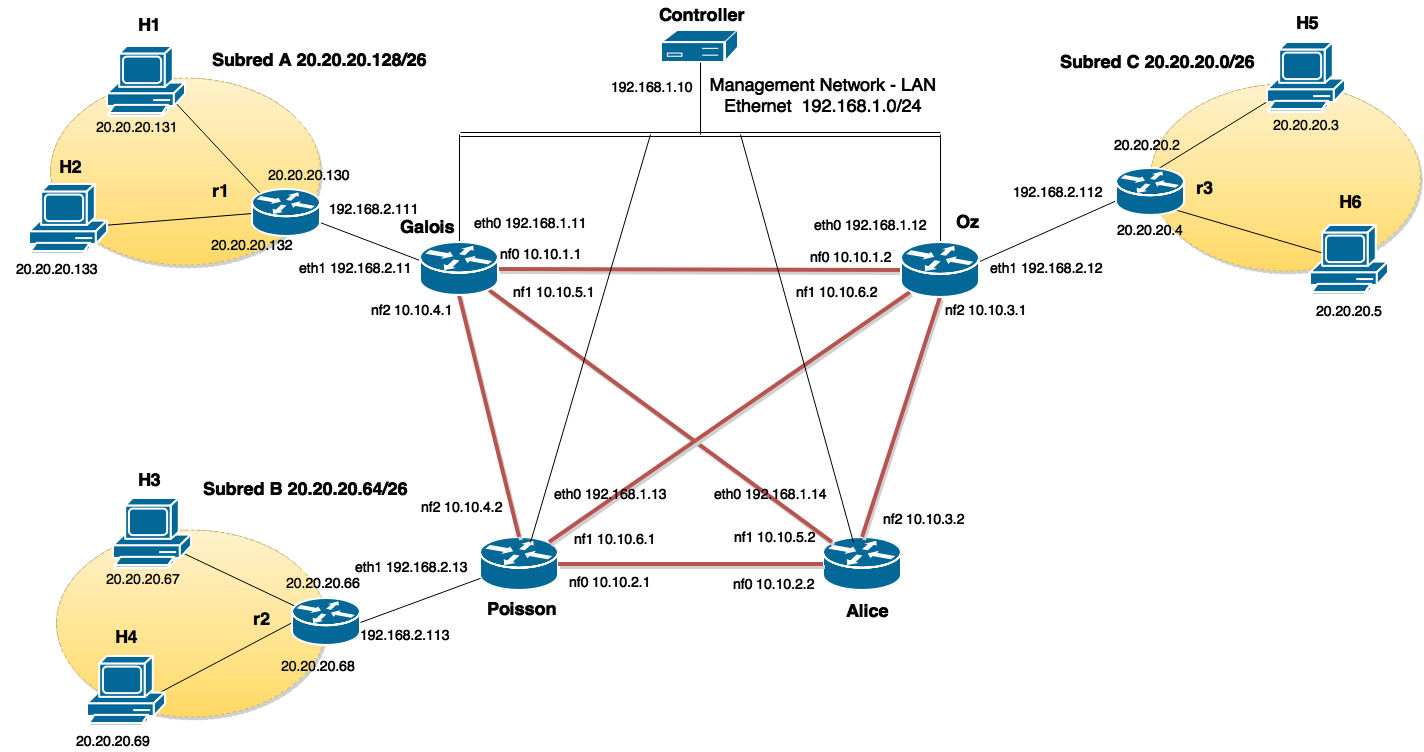
\includegraphics[width=1.0\textwidth]{CU1P1}
\caption[VPN de capa 3 - Escenario 1]{VPN de capa 3 - Escenario 1}
\label{fig:CUP1}
\end{figure}

Sobre este escenario se van a ejecutar una serie de pruebas orientadas a verificar los siguientes aspectos en el prototipo:

\begin{enumerate}
\item Clasificaci\'on de tr\'afico
\item Algoritmo de ruteo
\item Algoritmo de distribución de etiquetas
\item Actualizaci\'on de rutas cuando cambia la topolog\'ia
\item Capacidad para crear VPN multipunto
\end{enumerate}

Con el objetivo de comprobar estos aspectos se crean los siguientes servicios:

\begin{center}
\begin{tabular}{| l | l | l | p{4cm} | p{4cm} |}
\hline
Nombre & Ingreso & Egreso & Clasificación & Descripción \\ \hline

\crule[Aquamarine]{0.3cm}{0.3cm} S1 & Galois - eth1 & Oz - eth1 & ip\_src=20.20.20.128/26 ip\_dst=20.20.20.0/26 & Tr\'afico de Subred A a Subred C \\ \hline

\crule[Red]{0.3cm}{0.3cm} S2 & Oz - eth1 & Galois - eth1 & ip\_src=20.20.20.0/26 ip\_dst=20.20.20.128/26 & Tr\'afico de Subred C a Subred A \\ \hline

\crule[ForestGreen]{0.3cm}{0.3cm} S3 & Galois - eth1 & Poisson - eth1 & ip\_src=20.20.20.128/26 ip\_dst=20.20.20.64/26 & Tr\'afico de Subred A a Subred B \\ \hline

\crule[LimeGreen]{0.3cm}{0.3cm} S4 & Poisson - eth1 & Galois - eth1 & ip\_src=20.20.20.64/26 ip\_dst=20.20.20.128/26 & Tr\'afico de Subred B a Subred A \\ \hline

\crule[RoyalPurple]{0.3cm}{0.3cm} S5 & Poisson - eth1 & Oz - eth1 & ip\_src=20.20.20.64/26 ip\_dst=20.20.20.0/26 & Tr\'afico de Subred B a Subred C \\ \hline

\crule[YellowOrange]{0.3cm}{0.3cm} S6 & Oz - eth1 & Poisson - eth1 & ip\_src=20.20.20.0/26 ip\_dst=20.20.20.64/26 & Tr\'afico de Subred C a Subred B \\ \hline

\end{tabular}
\end{center}

Para cada uno de estos servicios adem\'as se indica el etherype 0x0800 correspondiente al tipo de tr\'afico IPv4.

\begin{itemize}
\item S1: <Subred A, Subred B>
\end{itemize} 
\newpage
\subsection{Escenario 2}

Este escenario representa una red privada punto a punto de capa 3. Esta compuesto por dos organizaciones diferentes, cada una de ellas con dos sucursales f\'isicamente separadas.

Se quiere instancia entonces servicios en RAUFlow con el objetivo de brindar conectividad entre cada par de sucursales.
 
\begin{figure}[ht!] 
\centering    
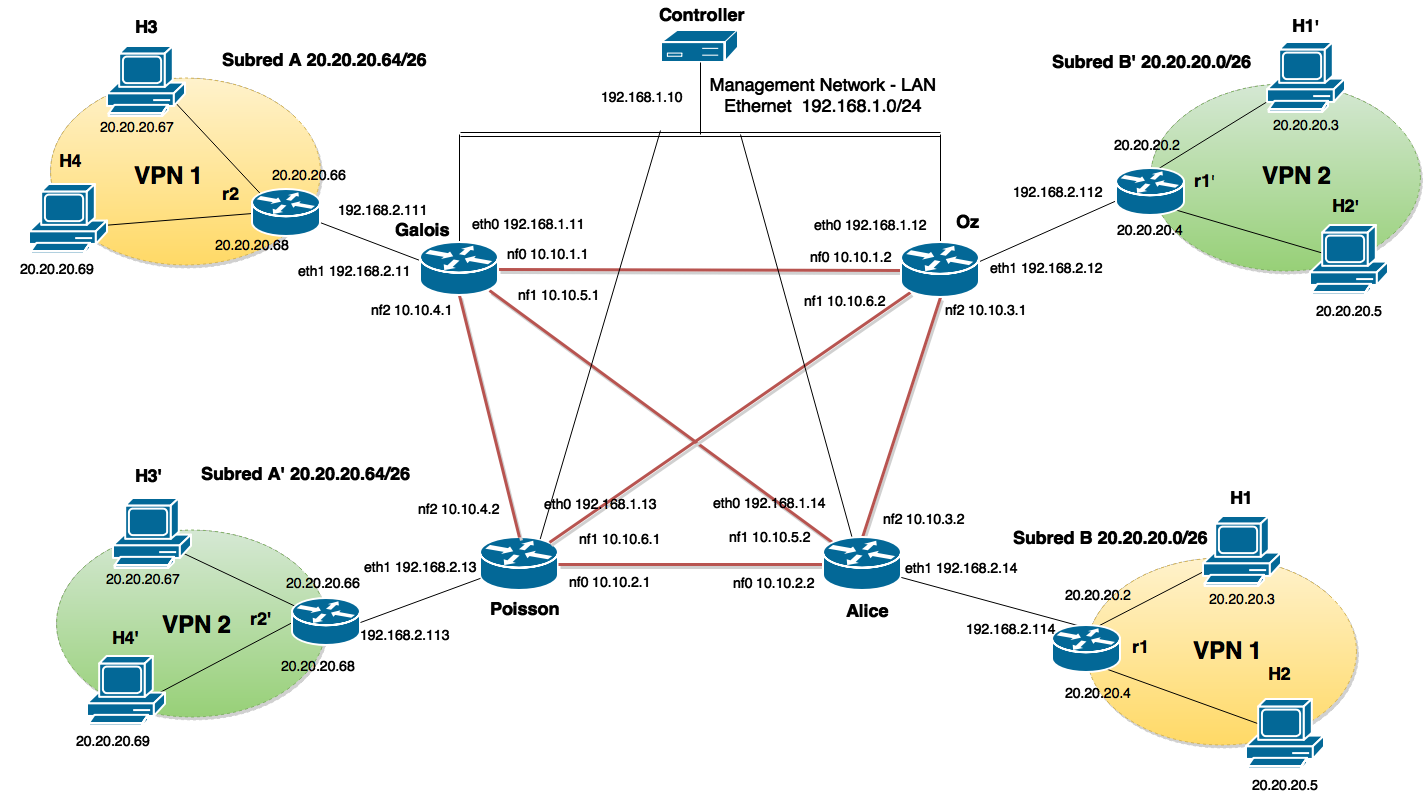
\includegraphics[width=1.0\textwidth]{CU1P2}
\caption[VPN de capa 3 - Escenario 2]{VPN de capa 3 - Escenario 2}
\label{fig:CUP2}
\end{figure}

\section{Pruebas}

\subsection{Asignación de etiquetas}

\subsubsection{Objetivos}
\begin{enumerate}
\item Probar que el algoritmo de distribución de etiquetas funciona correctamente en relación a: (a) asignación de etiquetas identificadoras a nuevos servicios(segundo nivel de etiquetas) y (b) asignación de etiquetas a caminos LSP.
\item Analizar el comportamiento de este algoritmo cuando se prueba con un rango amplio de etiquetas dentro del espacio de etiquetas disponible.
\end{enumerate}

\subsubsection{Descripción de la prueba:}
[Crear muchisimos servicios para utilizar gran parte del arango de etiquetas disponibles. Tomar un muestreo de servicios que utilicen etiquetas que creamos convenientes y analizar el comportamiento del prototipo para el trafico generado en estos servicios en:]

\begin{itemize}
\item Trafico asociado a una VPN es correctamente etiquetado a la entrada del prototipo
\item Trafico asociado a una VPN sale de la red del laboratorio por el nodo de salida y la interfaz de salida prevista, sin etiquetas.
\end{itemize}

\subsubsection{Resultados obtenidos:}

\subsection{Clasificación de tr\'afico}

\subsubsection{Objetivos}
\begin{enumerate}
\item Verificar la clasificación de trafico en base a los matching fields de OpenFlow en los nodos de ingreso
\item Verificar la clasificación de tr\'afico en función a los campos puerto de entrada y etiqueta en los nodos internos(LSRs)
\end{enumerate}

\subsubsection{Descripción de la prueba}
[Hacemos capturas de pantalla en nodos de entrada y en nodos del medio para ver que el trafico se clasifica correctamente. Para esto debemos crear varios servicios]

\subsubsection{Resultados obtenidos}

\subsection{Algoritmo de ruteo dinámico}

\subsubsection{Objetivos:}


\subsubsection{Descripción de la prueba:}


\subsubsection{Resultados obtenidos:}


\subsection{Numeraciones superpuestas}

\textbf{Objetivos}

\textbf{Descripción de la prueba}

\textbf{Resultados obtenidos}